\documentclass{article}
\usepackage{url}
\usepackage{amsmath}
\usepackage{listings}
\usepackage[utf8]{inputenc}
\usepackage{fancyhdr}
\usepackage[font=footnotesize,labelfont=bf]{caption}
\usepackage{xcolor}
\usepackage{caption}
\usepackage{graphicx}
\usepackage{algpseudocode}
\usepackage{float}
\usepackage{lipsum}
\usepackage[english]{babel}
\usepackage{libertinus}
%\usepackage{libertinust1math}

% === Hyperlinks ===
%\hypersetup{
%    colorlinks=false,
%    linktoc=all
%}
% === End Hyperlinks ===

% === Colours ===
\definecolor{codegreen}{rgb}{0,0.6,0}
\definecolor{codegray}{rgb}{0.5,0.5,0.5}
\definecolor{codepurple}{rgb}{0.58,0,0.82}
\definecolor{backcolour}{rgb}{0.95,0.95,0.92}
\definecolor{dark}{rgb}{0.12,0.12,0.14}
%\pagecolor{dark}
%\color{white}
% === End Colours ===

% TODO: Configure page layout to conform to requirements.
% === Layout ===
%\setlength{\parskip}{0.5em}
\graphicspath{ {./images/} }
\lstdefinestyle{code}{basicstyle=\ttfamily\footnotesize, breakatwhitespace=false,
    breaklines=true, keywordstyle=\color{magenta}, commentstyle=\color{codegreen},
    keepspaces=true, showspaces=false, showstringspaces=false}
\lstset{style=code}
\pagestyle{fancy}
\fancyhf{}

\rhead{Callum Donovan}
\lhead{Implementing SAT Algorithms in Software}
\rfoot{Page \thepage}
\lfoot{CS-M20 - 1915769}
\title{\bfseries Implementing SAT Algorithms in Software}
\author{Callum Donovan}
\date{ \today }
% === End Layout ===

\begin{document}

% === Title Page ===
\begin{titlepage}
    \begin{center}
        \Large{\bfseries Implementing SAT Algorithms in Software} \\
        \vspace*{\fill}
        \begin{center}
            
\includegraphics[scale=0.15]{swan.jpg}
        \end{center}
        \vspace*{\fill}
        \bfseries{\large Callum Donovan \\
            1915769 \\
            \today \\
            Swansea University \\}
    \end{center}
\end{titlepage}
% === End Title Page ===

% === Main Content ===
\thispagestyle{empty}
\begin{center}
    \section*{Abstract}
\end{center}
% TODO: Use the word "implement" a lot less!
%The Boolean Satisfiability Problem is a fundamental part of Computer Science. First proven to be an
%NP-Complete problem by both Stephen Cook in 1971\cite{scook}, and Leonid Levin in 1973\cite{levin}. Since then, many more
%NP-Complete problems have been identified, along with their respective uses in the real world
%outside of pure computer science. Due to this, there has been a growing need for solvers that can
%effectively and efficiently process these problems. In the last two decades alone, huge progress has
%been made to coincide with the advancements in technology. And more SAT solvers have appeared that
%can be deployed in industries where they are most needed.

%This paper explores the basic concept behind SAT solvers, and how they can be implemented in
%software using modern programming languages and tools. The algorithm that will be
%implemented is one proposed by Donald Knuth in his book "The Art of Computer Programming". Knuth proposes
%many algorithms, ranging from the most basic backtracking based algorithm, to an advanced
%implementation of WalkSAT[!]. We will explore the fundamentals of how to implement these algorithms,
%implement one of them, then test its performance against a suite of SAT problems.

%The result of this paper will be a SAT solver implemented in C++, using the data structures and
%steps provided by Donald Knuth in his book "The Art of Computer Programming".

\newpage
\thispagestyle{empty}
\tableofcontents

\newpage
\section{Introduction}
% TODO: Refactor to sound better.
% TODO: Add some examples to interest the reader.
Satisfiability has presented itself a huge area of research throughout the history of computer
science. Being the first proved to be NP-Complete in 1971\cite{scook}, it has been the go-to for complex
computation. And using reduction techniques pioneered in the mid-twentieth century, many other types
of complex problems can be converted into SAT and solved using the plethora of solvers freely
available. In more recent years, SAT competitions have added an incentive to the development of more
advanced solvers, such as Minisat, zChaff, and CaDiCaL. On top of these, parallel solvers have
gained popularity and one such solver, called Plingaling, ranked very highly in the SAT Competition
2020. Showing how parallel solvers can be just as good as their counterparts, if not better.

Donald Knuth has taken particular interest in this topic with his recent chapter of "The Art of Computer Programming". He 
discusses how important SAT solvers are to both industry and research, as well as providing algorithms and sample problems to 
test them against.

This paper will be an exploration into the world of SAT solvers and how they can provide crucial services to both industry and 
research. As well as methods in which proposed SAT solver algorithms can be implemented into a robust piece of software. Due to 
the sheer size of literature and research in this field, it would be unrealistic to think it is possible to cover everything in a 
comprehensive way. Therefore, this paper focuses on the fundamentals of SAT and the significant research through the years since 
Cooks paper in 1971\cite{scook}. As well as the ideas presented by Donald Knuth for implementation in modern programming 
languages.

\subsection{Motivation}
The motivation behind this project stems from the ever growing need for more efficient and faster SAT solvers. But in order to 
begin researching in this field, one must know the basics and tried methods present today. This project will do just that, in 
both studying literature that has formed the basis of most of the field, and implementing a basic SAT solver.

One of the most common arguments for the research into SAT solving is its viability for both science and industry. This presents 
a convenient compatibility between the two. As industry requirements grow, so too does the need for research into better 
algorithms to satisfy those requirements. An example in which SAT solvers are a key part of industry include Electronic Design 
Automation (or EDA). We will explore these usages further as we progress and highlight the advantages of fast SAT solvers when 
applied to these industries.

Another common viability for SAT solvers includes their usage for most complex problems that can be reduced to SAT. Most problems 
in the real world can be cast as optimisation problems. This allows us to create a mathematical description of these problems, 
which in turn can present themselves for solving. The use of a solver in this instance would produce results which would allow 
for cost-saving or general efficiency improvements.

\subsection{Aims and Objectives}
% TODO: Refactor this section, especially the DK bit.
To preface this project we must present the aims and objectives that we wish to aim for. As explained above, we do not wish to 
push the boundaries of SAT solvers in this particular project. But instead want to explore the basics and expand on current 
research. Aiding us in this goal will be the series by Donald Knuth, "The Art of Computer Programming". Knuth has recently taken 
interest in the concept of satisfiability for "Fascicle 6: Satisfiability" , and presents a large amount of content for us to 
analyse. In this book, Knuth outlines multiple algorithms that could be used to implement multiple common SAT solvers\cite{donald}
. These include:

\begin{itemize}
    \item Algorithm B - Backtracking with watched literals.
    \item Algorithm D - DPLL.
    \item Algorithm C - CDCL.
    \item Algorithm L - DPLL with lookahead.
    \item Algorithm W - WalkSAT.
\end{itemize}

% Be careful of the spell checker attempting to "americani(z)e" everything.
We shall be analysing one of these algorithms and presenting the data structures needed and methods of implementation using C++. 
Once our implementation is complete, and testing has proved the solver to be working as intended, we will record the performance 
metrics in a scientific manner to ensure accuracy. These metrics will then be compared to other FOSS solvers that are well tested 
and commonly used. This will give us a benchmark as to how increasing complexity of the algorithm and program can achieve greater 
performance. As well as how the programming language chosen can effect the overall performance.

We can easily turn these actions into functional and non-functional requirements. Doing so will allow us to test against the 
requirements stated and compare the expected result to the actual result. This format matches a more "software engineering" 
approach, which is desired for this project.

\subsubsection{FREQ1}
The resulting software should be able to process an input CNF formula in the semi-standard DIMACS format.

\subsubsection{FREQ2}
% TODO: Clarify this, 'short amount of time' doesn't seem very scientific.
The resulting software should be able to evaluate the satisfiability of a simple formula from FREQ1, and return the result when 
found. Simple refers to a formula which most SAT solvers would be able to process in a short amount of time. Result refers to the 
decision returned from the solver that concludes as "SATISFIABLE" or "UNSATISFIABLE".

\subsubsection{Non-Functional Requirements}
These requirements differ from functional requirements as they are not crucial to the project's success. These are simply goals 
that, if time allows, can be implemented for further data.

\subsubsection{NFREQ1}
The resulting software should be able to process a complex formula within a reasonable amount of time. Reasonable refers to the 
length of time it takes to return a result when compared to other SAT solvers, i.e. 300 seconds to return "SATISFIABLE".

%\begin{itemize}
%    \item To make a SAT solver using instructions from "TAOCP"
%    \item Make sure the solver can solve generic problem sets in DIMACS.
%    \item Make sure the solver can do this in a decent amount of time.
%    \item Basically FREQ1 and FREQ2.
%\end{itemize}

\section{Background}
Before we get into the implementation and software, it is always good to have a solid understanding
of the topic at hand. SAT in particular is quite a deep topic, it is easy to spend a long time
researching into all the intricacies[!]. For this project, we will just be concentrating on the
general concepts and ideas behind the most common instances of SAT. Along with some deep diving when required to ensure we
understand what we're trying to achieve.

% TODO: Insert previous CSCM10 research here, cause we ain't doing it again!

\subsection{P vs NP}
Before we progress into the basics of SAT, we can quickly explore the reason behind it being such an
important topic within computer science. The P vs NP question is one of the most prevalent in the
field of complexity theory. It is one of the seven millenium prize problems put forward by the Clay
Mathematics Institute and, if solved, fetches a \$1 million prize for the first correct solution.
The concept of P vs NP asks whether every problem whose solution can be verified quickly, can also
be solved quickly. On the surface sounding simple, but in the details an incredibly hard question
that has plauged computer scientists since the 1950s.

% TODO: Expand on NP-Complete using previous research.
A further interest within this field of study concerns the notion of NP-Complete.

The Boolean Satisfiability Problem was the first to be proven NP-Complete, by both Steven Cook and
Leonid Levin in 1971 and 1973 respectively\cite{scook}\cite{levin}. It was later included in a
well-known paper, \textit{Reducibility Among Combinatorial Problems} by Richard Karp\cite{karp},
which generated a renewed interest amongst researchers. In this paper, Karp proved how a large
set of problems could be reduced to an instance of SAT. Thus meaning each one would be solvable if
there was a suitable algorithm. The faster algorithm that we can create for the SAT problem, the
better we can solve other problems via reducibility.

\subsection{Boolean Satisfiability Problem}
%\begin{itemize}
%    \item Define the SAT problem with reference.
%    \item Explain how SAT formulas are constructed.
%    \item Explain early attempts to solve SAT formulas.
%    \item Discuss the DPLL algorithm, the first computer implementation of a solver.
%\end{itemize}
As stated by Donald Knuth, the Boolean Satisfiability Problem is defined as such:

% TODO: Add citation for this quote. Also make this look a bit better...
\begin{quotation}
    "Given a Boolean Formula $F(x_1,...,x_n)$, expressed in so called "conjunctive normal form" as an AND of ORs, can we "satisfy" $F$ by assigning values to its variables in such a way that $F(x_1,...,x_n)$ = 1?"
\end{quotation}

Given this definition, we can present a formula as detailed above:

\begin{center}
    $F(x1,x2,x3) = (x_1 \vee \bar{x_2}) \wedge (x_2 \vee x_3) \wedge (\bar{x_1} \vee \bar{x_3}) \wedge (\bar{x_1} \vee \bar{x_2} \vee x_3)$
\end{center}

And given this formula, we can satisfy it by setting $x_1x_2x_3 = 001$.

To ensure consistent understanding of these concepts before proceeding, we can simplify the notation
for each element within SAT. To begin, we have \textit{variables}. These are elements of any
convenient set. Variables can be denoted in a few ways, but for this we shall be using Knuth's own
notation as stated in his book. Thus, variables will be denoted using numerals $1, 2, 3, ...$ to save
having to repeat characters. We can also omit the brackets and operators to make the writing of
formulas much faster:

\begin{center}
    $R = \{12\bar{3},23\bar{4},341,4\bar{1}2,\bar{1}\bar{2}3,\bar{2}\bar{3}4,\bar{3}\bar{4}\bar{1},\bar{4}1\bar{2}\}$
\end{center}

\textit{Literals} are our next notation. They correspond to either a variable or the compliment of
that variable. Using our previous example for variables, if $1$ is a variable, both $1$ and
$\bar{1}$ are literals. From this we can easily deduce that if there are $n$ number of variables,
there can be $2n$ possible literals. A literal may be considered \textit{pure} if its negation does
not appear anywhere in the formula. And thus can be safely set to true or false respectively.

There are multiple instances of the satisfiability problem, so we shorten satisfiability to just
SAT. In turn, each instance is typically abbreviated and prefixed to SAT. Examples of this would
be 2SAT, 3SAT, and $k$SAT.

There are more definitions which represent alternative types of clauses that we could encounter. For  instance, a clause of 
length 1 is called a \textit{unit clause}. Clauses of length 2
would be called \textit{binary clause}, length 3 \textit{ternary clauses}, and so on. We can also
encounter clauses in which there are no literals, which would be called \textit{empty clauses}.
\textit{Empty clauses} are denoted using $\epsilon$ and are always unsatisfiable. As you might
think, shorter clauses would be easier to satisfy as they contain less literals, but this is not
necessarily the case. As we progress further into the design and implementation of this solver, we
will learn the importance of covering all bases and making no assumptions of difficulty.

% TODO: Figure out a better name for this heading.
\subsection{Polynomial Time Reduction}
There are a plethora of problems that can be formulated into the previously stated problem. It is
for this reason that we find the field of SAT solvers so important. Karp\cite{karp} introdeced the idea of converting alternative
problems to the SAT problem via \textit{Polynomial Time Reduction}.
% TODO: Expand on this.

\subsection{Complete vs Incomplete SAT Methods}
Before we progress onto the details of SAT algorithms, we must understand the two distinct types of
solvers; complete and incomplete. Currently we are most interested in the former of the two, as it
presents the best usage out of all the problems that are faced within SAT. A complete SAT algorithm
is one that finds both satisfiable and unsatisfiable solutions, and returns the corresponding model
if satisfiable.

Modern SAT solvers are almost all complete and incorporate the original DPLL algorithm. They are extended using modern techniques
to significantly speed up the solving process, and in most cases are capable of solving problems with millions of variables.
Examples of some modern complete SAT solvers are Minisat and CryptoMiniSat. As we will detail below, these are two interesting
solvers that are designed for particular purposes.

Incomplete solvers are much more rare compared to their complete counterparts. The obvious reason being that they do not return a
result that we would be satisfied with, as they do not report if an instance of SAT is unsatisfiable. Aside from this, they do 
have their uses for specific types of SAT problems, hence why they are still being developed today. An example of an incomplete 
SAT solver is \textit{WalkSAT}. WalkSAT is based on a local search algorithm which tries to find a satisfying assignment by 
iteratively improving on them until all constraints are satisfied.

\subsection{DPLL Algorithm}
The DPLL algorithm is one of the most important milestones in the history of SAT. Itself being a further development of work by 
Martin Davis and Hilary Putnam in their 1960 paper \textit{A Computing Procedure for Quantification Theory}\cite{putnam}, the 
DPLL algorithm attempted to take this initial work and refine it.
% TODO: Maybe talk about Herbrands Theorem here too?

The DPLL algorithm still forms the basis of most efficient SAT solvers today. Each instance of a SAT solver that utilises the 
original DPLL algorithm typically adds their own optimisations and improvements to achieve a greater efficiency, something we 
will expand on in further sections. In simplified terms, the backtracking section works by choosing a literal, assigning a truth 
value to it, simplifying the formula then checking if the new simplified formula is satisfiable. If this is the case the solver 
will return that the original formula is satisfiable and return the model. If this is not the case, the solver will backtrack and 
assign the opposite truth value and run the above checks again. The improvements made to this basic backtracking approach include 
adding rules to each step for enhanced performance. These rules are:

\begin{itemize}
    \item Unit Propagation.
    \item Pure Literal Elimination.
\end{itemize}

The former capitalises on \textit{unit clauses} to avoid a large section of the search space. By finding a unit clause, the 
solver will then assign the appropriate truth value to the literal to make it true, making these clauses trivial.

The latter capitalises on variables which only appear in one form throughout the forumula, a \textit{pure literal}. If this is 
the case, clauses in which this pure literal appear can be safely assigned in a way that makes all clauses they are contained in 
true. Doing this means the solver can safely delete the clauses where this is the case and further reduce the search space.

\subsection{Modern SAT}
%\begin{itemize}
%    \item Talk about how SAT has evolved since the original DPLL.
%    \item Modern SAT competitions.
%    \item Parallel SAT solvers.
%    \item General future SAT solver stuff.
%\end{itemize}
Since the original instances of SAT there has been an astonishing amount of development into
faster and more efficient methods. Since the milennium alone SAT solvers have managed to keep up
with the quickly advancing hardware, allowing for the processing of SAT problems with sometimes up
to millions of clauses. Alongside the state of the art solver have also been attempts to simplify
methods used in software, to try and help people just getting into the topic. Solvers such as
\textit{Minisat} were designed to be as small and simple as possible, whilst still incorporating
advanced techniques for maximum efficiency.

Alongside these advancements has been the annual SAT competition. This competition collates the
latest and greatest work from the field and tests it against a plethora of advanced problems to see
who comes out on top. For researches, or even hobbyists, being the victor of one of these
competitions is an astonishing achievement. But there is more to the competition that just the
prize. Multiple categories within the competition have allowed for more experimental ideas to come
to fruition. Such examples as \textit{Lingeling, Plingeling,} and \textit{Treengeling} capitalise on
the notion of parallelism and attempt to drastically speed up processing times. This is of course
easier said than done, and prove that achieving efficient parallelism in SAT is quite a challenging
task. As parallelism is becoming a key part of modern processor technology, it is integral to the
development of software such as SAT solvers to exploit high core counts. As for SAT, there are a few
ways one can go about this.

\textit{Portfolio} SAT solvers are composed of multiple solvers that are all good at tackling
different types of problems. As there is no single solver that is better at all problems than all
others, it makes sense to apply each solver to a part of the problem that it is best at. For
instance, we can collate some of the most competitive solvers into a single \textit{portfolio}, and
feed all of them the same problem. Once one of the solvers returns their result, all the others will
also terminate. As you can imagine, this would lead to a large amount of duplicate processing. And
whilst this is true, the advantage is that applying the problem to all these solvers will still be
competitive, as the range of solvers will increase the chances of finding a solution in the fastest
time possible. As with most parallel workloads, the downside to this is that the machine running
these solvers will have to posess a large amount of memory. An example of an effective portfolio
style solver is \textit{HordeSat}[!], which is capable of almost linear speedup depending on the
problem set. % TODO: Maybe add some proof of this speedup here?

\section{Related Work}
Moving on from the background of SAT, we can look into existing solutions that are freely available.
As of 2020, there are plenty of FOSS programs that can be used to solve large sets of problems. This
is in part due to the regularity of the SAT competitions that encourage people to build
groundbreaking solvers.

\subsection{Current Research}
\subsubsection{CDCL}
Although it may feel like progress in this field can be quite slow, there is constantly ongoing research into methods in which we
can improve the existing methods. Typical DPLL based solvers iteratively improve by including extra features that solve individual
problems, such as look-ahead. Other research has suggested altering the traditional DPLL algorithm to be utilised on other
problems such as \textit{satisfiability modulo theories}. In this instance, an extension of the DPLL algorithm was created called
\textit{DPLL(T)}. Put simply, this version of the algorithm transforms an SMT problem into a SAT formula where atoms are replaced
by boolean variables. Modern SAT goes a step futher by implementing advanced features such as \textit{clause learning} and
\textit{back jumping}, more taking inspiration from the original DPLL algorithm as opposed to iterating on top of it. The
resulting algorithms are called \textit{conflict-driven clause learning} and present a massive improvement over traditional DPLL
based solver.

\subsubsection{NeuroSAT}
But aside from these developments, there is still alternative research being done to approach the SAT problem in different ways.
One such instance of this is \textit{NeuroSAT}, a SAT solver that utilises neural networks to power its internals. Although proven
to not be anywhere near as performant as state-of-the-art SAT solvers, such as the ones mentioned above, it lays the foundation
for the potential use of machine learning and AI in the world of SAT. As we have all come to expect in Computer Science, machine
learning can sometimes be considered a buzzword for a lot of things that amount to nothing. However, NeuroSAT has been able to
solve substantially larger SAT instances than it had been trained on[!]. Thus proving to be quite promising in concept and
sparking interest in its potential. Although the concluding remarks of this paper suggest that there is no obvious way forward
from this concept, it seems that it could potentially be something that could be learned from as a method of approaching SAT from
a different direction.

\subsection{Popular SAT Solvers}
\subsubsection{Minisat}
A popular and early solver that has won many competitions[!] is Minisat. Written in C++ and boasting
just a mere few hundred lines of code, Minisat has been proven to be an effective tool for medium
sized problem sets. First written in 2003 by Niklas Een[!] and Niklas Sorensson[!], its primary goal
was to help developers and researchers get into the field of SAT solving by providing a simple
interface and minimal codebase.

%\begin{itemize}
%    \item Talk about Minisat.
%    \item Go into detail about offshoots from Minisat, such as CryptoMiniSat.
%    \item Newer CDCL algorithms.
%    \item Look into SAT 2020 to find some interesting new solvers.
%    \item Basically talk about applications then the research currently happening.
%\end{itemize}

\subsubsection{CryptoMiniSat}
CryptoMiniSat is an advanced, modern SAT solver created by Mate Soos, Karsten Nohl, and Claude Castelluccia\cite{cryptominisat}.
As the name suggests, this solver builds upon the foundations laid by Minisat to create an all in one solution to multiple 
problems. CryptoMiniSat implements most of the useful features from Minisat 2.0 core, along with PrecoSat and Glucose to try to 
make a one-stop solution. CryptoMiniSat is still in active development, hosting their code on GitHub for open collaboration. This 
solver is the work of massive proportions and contains a extensive list of features to try to make as efficient a solver as 
possible. Based off of their 2009 conference paper \textit{Extending SAT Solver to Cryptographic Problems}, it contains over 50,
000 lines of code as opposed to Minisat's 1,500. As stated in the projects FAQ, one of its main aims from the offset was to apply 
SAT solvers to cryptographic problems. However this ended up being just one of the many types of SAT that it excelled at.

% TODO: Finish this section
\subsubsection{Chaff / zChaff}
\lipsum[2-3]
\subsubsection{GRASP}
\lipsum[2-3]

\subsection{Limitations}
It can be quite challenging to come up with potential limitations for state-of-the-art solvers. But, when generally speaking,
there is always potential for improvement based upon the advancements in computer hardware. Many SAT solvers nowadays are already
more than good enough for industrial purposes. They are something that would have been merely dreamed of when the DPLL algorithm
was first created. But as we go ahead into a promising future filled with technological innovations, such as the rise of quantum
computing or alternative methods of constructing the transistor, we can be sure that further innovations with SAT will follow.

\section{Design}
%\begin{itemize}
%    \item Summary of what we would want from a design.
%    \item Include the algorithm from Donald Knuth (algorithm D).
%    \item Discuss the data structures that we will need to implement based off of DK's ideas.
%\end{itemize}
The following section will include analysing and detailing the algorithms presented by Knuth. This will include both
\textit{Algorithm D} and \textit{Algorithm L}, both of which are representitive of modern DPLL solvers. We will flesh out the
general structure to be translated into code and investigate the required data structures along with how they can be implemented
in our chosen language.

\subsection{Base Algorithm}
The key to all the most successful SAT solvers is the algorithms. The first SAT solver to be implemented for a computer used the
DPLL algorithm[!]. As we previously established, the DPLL algorithm is considered one of the firsts and produced good results for
the time. As of the last decade, there have been a plethora of improvements to the original DPLL algorithm that has allowed it to
keep up with the increasing complexity of problems available. The general pseudocode for the original DPLL algorithm can be
written as such:

\begin{figure}[h]
    % TODO: Put the DPLL algorithm pseudocode here
    % Fix the notations not showing up!
    \centering
    \begin{lstlisting}[language=C++]
    Algorithm DPLL
        Input: A set of clauses C
        Output: A truth value

    Function DPLL(C)
        if C is a consistent set of literals then
            return true;
        if C contains an empty clause then
            return false;
        for every unit clause {L} in C do
            C ← unit-propagate(L, C);
        for every literal L that occurs pure in C do
            C ← pure-literal-assign(L, C);
        L ← choose-literal(C);
        return DPLL(C AND {L}) or DPLL(C AND {not(L)});
\end{lstlisting}
\end{figure}

\subsection{Data Structures}
Before we progress to the next algorithms, it is important that we establish the data structures we will be needing. Knuth
outlines the data structures that are important to these specific algorithms, and explains how their usefulness depends on how
they are implemented. For his introduction to \textit{Algorithm B}, Knuth proposes that we use \textit{watched literals}. This
concept details that we only need to keep an eye on the relevent literal per clause at any one time[!]. Using this notion, Knuth
proceeds to heavily simplify his original data structures from \textit{Algorithm A}, and achieving an impressively small
procedure that is still capable of solving small to medium sized problems.

For our case however, we will be utilising both the lazy data structure that Knuth proposes for \textit{Algorithm B}, and combine
it with a method of capitalising on \textit{unit clauses}. Knuth details that we can extend the data structures from \textit{Algorithm B} by introducing indicies $h_1...h_n$.

% TODO: Actually talk about the damn data structures!

\subsection{Algorithm D - SAT by Cyclic DPLL}
Knuth presents multiple algorithms to us in his book, but for this project are interested in specifically two of them. Algorithm D
is the first we shall analyse, which will lay the foundation for Algorithm L.

% TODO: FIX THIS! NOT THE ALGORITHM WE ARE USING ANYMORE!
For our project, the algorithm that we will be interested in is a general DPLL algorithm. As
previously discussed, this is just one of a few algorithms given from Donald Knuth. Although it is
relatively simple, it is a good way to explore the basic idea of software SAT solvers. Forming a
foundation for possible further improvements, much like those explained in algorithm L. Donald Knuth
describes the algorithm in a series of steps, also outlining the data structures that we need to
implement it as he has described. The following is the algorithm steps that are detailed by Knuth in his book:

% TODO: Finish adding this.
\begin{enumerate}
    \item Set $m_0 \leftarrow d \leftarrow h \leftarrow t \leftarrow 0$, and do the following for $k = n, n - 1, ..., 1:$ Set $x_k ← -1$ (denoting an unset value); if $W_{2k} \neq 0$ or $W_{2k+1} \neq 0$, set \texttt{NEXT}($k$) $ \leftarrow h, h \leftarrow k$, and if $t = 0$ also set $t \leftarrow k$. Finally, if $t \neq 0$, complete the active ring by setting \texttt{NEXT}($t$)$ \leftarrow h$.
    \item Terminate if $t = 0$ (all clauses are satisfied). Otherwise set $k \leftarrow t$.
\end{enumerate}

Knuth names this algorithm "\textit{Algorithm D - Satisfiability by Cyclic DPLL}. It is based on the
original algorithm presented by Martin Davis, George Logemann, and Donald Loveland\cite{dpll},
extending previous work Davis did with Hilary Putnam[!]. At the time of it's inception, this
algorithm was seen as fantastic. But due to limitations of the hardware, their methods of storing
and processing data were quite verbose. It involved having to record all the data of the current
node onto a magnetic tape before branching. When they wished to backtrack to the previous node,
they would restore the data from the tape they had created. But now we have huge stocks of memory
available to use whenever necessary, allowing us to write more complex and faster solvers using
equally more complex data structures.

\subsection{Algorithm L - Utilising Lookahead}
Knuth further expands on the previous algorithm by implementing a procedure called \textit{look-ahead}. This procedure attempts to determine the best direction in which to branch by performing \textit{look-ahead} on a set of variables, then evaluating the resulting reduction of the formula. Put simply, the \textit{look-ahead} procedure attempts to predict the future for the success of the present.

%\begin{itemize}
%    \item Discuss algorithms presented by DK.
%    \item Discuss which algorithm we are planning to implement.
%    \item Talk about the ones we aren't going to anyway?
%\end{itemize}
% TODO: Talk about how we've design the code based off of the algorithm and preceding content in the book.

\section{Implementation}
%\begin{itemize}
%    \item Discuss the general idea of the program, including inputs (DIMACS) and outputs (SAT / NON-SAT).
%    \item Discuss the process in which we are going to be solving these problems.
%    \item Talk about our tool-chain and related crap.
%    \item Talk about the attempts at implementing it.
%    \item Show the final implementation.
%\end{itemize}

The following will be an in-depth look at the steps we need to consider when implementing our
project. Following the design, this section details the general input and output of the program. As
well as the processing that forms the core of the solver. We will also outline the data structures
that are to be implemented and how they will be integrated with the algorithm to culminate in a
working SAT solver.

We will also be glazing over the tool-chain and related items that are to be used to create the
solver. This includes the language and the compiler that will be used. As well as the editor and
reasoning behind these choices.

% TODO: Alter this title
\subsection{White Box}
% These are the basic steps of a computer program.
% Explain to the reader what is included for SAT.
\subsubsection{Input}
The input of the program will be a CNF formula presented in the DIMACS file format. This file format
is the standard for the SAT competitions and allows for simple parsing of the problem. The format
consists of few elements to ensure the problem is presented cleanly, the first of which being
comments. Comments can be marked using the character \texttt{'c'} followed by a single whitespace
character:

\begin{center}
    \texttt{c This is a comment line}
\end{center}

Lines prefixed with this will be treated as a
comment and thus will not be parsed as part of the problem. After the comments is a line telling the
SAT solver about the problem it is about to ingest, denoted using the character \texttt{'p'}
followed by a single whitespace character.

\begin{center}
    \texttt{p cnf 255 829}
\end{center}

This line will include the type of problem, followed by the number of clauses then
variables. Following the problem description line is the actual formula. This is presented by either
a positive or negative integer, terminated with a \texttt{'0'}.

\begin{center}
    \texttt{15 16 17 18 19 20 21 0}
\end{center}

Each line corresponds to a clause formatted in the defined problem type. And each integer represents
a unique variable. Using this format we can create consistent problem files which our solver will be
able to ingest and process easily. An example of a problem formatted in this format is presented
below:

% TODO: Get this to actually center
\begin{center}
    \begin{lstlisting}
        c pigeonhole 2 1
        c label:unsatisfiable
        c label:easy
        p cnf 2 3
        1 0
        2 0
        -1 -2 0
    \end{lstlisting}
\end{center}

This input will be read line by line by the solvers parser, recording the key information that it
needs. After successful parsing we can move on to the processing of this problem.

\subsubsection{Processing}
%\begin{itemize}
%    \item Discuss how the processing works.
%    \item This is the real meat that basically explains the algorithm.
%    \item I feel it would be best to at least discuss the DPLL algorithm.
%    \item Use content from TAOCP and online.
%\end{itemize}
This section details the bulk of what our program will do. Based off of Algorithm L dicussed in the design section, we will be
implementing it as closely as possible in modern C++. Our data structures will also be integral to how this part will operate, and
thus we must ensure we spend appropriate time to optimise them the best that we can.



% TODO: Explain how the algorithm processes our input.

\subsubsection{Output}
% https://web.archive.org/web/20190913185210/http://www.satcompetition.org:80/2004/format-solvers2004.html
%\begin{itemize}
%    \item The output will be "SATISFIABLE" or "UNSATISFIABLE".
%    \item Could also output the best solution.
%    \item Explain the output standard for SAT competitions.
%    \item SAT Competition 2002 output rules (see above comment).
%\end{itemize}

The output of our program is just as important as the input. After all, we want to know how the
solver has gotten to the solution it has ended at. Much like the input, we will be following a
semi-standard format that is outlined at each SAT competition. Using this format will allow us to be
consistent with how most SAT solvers output their solutions.

The format of the output is somewhat similar to the DIMACS format. In that each line is prefixed
with a single character denoting its purpose, followed by a single whitespace character. The main
difference here being that there is no particular order in which the lines must appear. There are
three distinct types of lines in this format:

\begin{itemize}
    \item \texttt{'c '}: Denotes a comment line in which the program can output any auxilliary
          information.
    \item \texttt{'s '}: Denotes the line where the solution is presented. This must be either
          'satisfiable', 'unsatisfiable', or 'unknown'. Only one instance of this line is allowed.
    \item \texttt{'v '}: Denotes the values of the solution if one is found.
\end{itemize}

The resulting output should combine all three of these types to create a comprehensive result to the
user. This includes the model that the solver has settled on if the solution is satisfiable. This
will allow for the checking of the answer to ensure its correctness.

\begin{figure}[h]
    \centering
    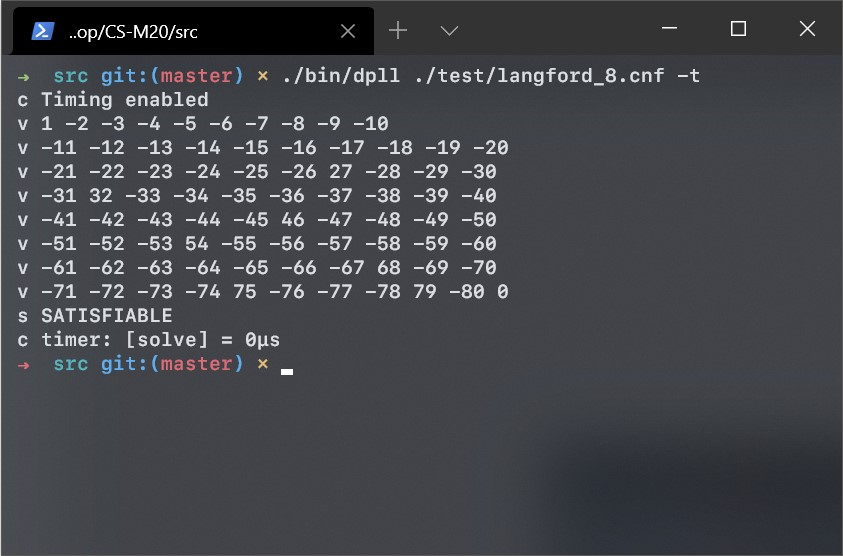
\includegraphics[width=0.8\textwidth]{output_example.jpg}
    \caption{Output format.}
\end{figure}

% This is going to be pretty important, attempt to simplify for the reader.
\subsection{Implementing the Data Structures}
%\begin{itemize}
%    \item Discuss why we're going to have to implement specific data types.
%    \item Provide examples on the types of structures to be used.
%\end{itemize}

The data structures that Knuth presents to us are not the easiest to implement in practice. As he mentions, programmers enjoy having clear and concise programs, but sometimes there needs to be complexity in order to achieve a specific goal. Because of this, the data structures for this algorithm ended up being rather complex to replicate with C++.

% TODO: Detail how the data structures are pretty complex.

\subsection{Tool-chain}
The following is a quick overview of the tool-chain that will be used for this project. As these aren't the meat of what the 
project is about, we shall only spend a short time glazing over the available solutions and those we picked.

\subsubsection{Compiler \& Libraries}
There are multiple compilers available for C++ dependant on the platform. Generally for each of the three most common platforms 
(Windows, Linux, and MacOS) there are reliable and well tested compiler suites available. The GNU Compiler Collection, or GCC, is
considered one of the standard compiler suites for C and C++. GCC has implementations for each of the aforementioned platforms 
via ports. The Windows implementation in particular is included in a few software development environments that are freely 
available; MinGW, MSYS2, and Cygwin.

As for Linux, the GCC suite can be installed natively typically using the preferred distro's package manager. For this project the
code will be compiled on a Debian based system using the GCC suite. Linux provides a simpler method of developing using C / C+
+ and streamlines the time from development to testing. Alongside this, the included GDB debugger allows for a simple and 
lightweight debugging solution. We will also be making use of bash scripts to invoke the software and provide flags to control 
options, something that can be a little more challenging on a Windows machine.

No development will be carried out on a Macintosh as we simply do not have access to one. Typically these types of software are 
compiled and run using a Linux system, and thus it would make the most sense to follow the given norm.

\subsubsection{Editor \& Environment}
There are a huge swathe of IDE's and editors available for use and as for which one to use, there isn't a definitive answer. We 
thought that it would be best to just stick with what we know best, and for this instance that would be Visual Studio Code. 
Although other IDE's are available that can take a lot of the work out of managing a project. It is not really necessary to use 
one here. This project will not contain a huge amount of code or files, and general debugging and profiling does not need to be 
done using bloated IDE's. Visual Studio Code contains a massive inventory of extensions available to give an experience just as 
rich as an IDE, but without the cumbersome nature of one. As for this project we only need a single extension to get the required 
development environment:

\begin{itemize}
    \item C / C++
\end{itemize}

It is also important to mention any other environment software aside from the previously mentioned. We are going to be using the 
\textit{time} command to accurately measure the time metrics of the software from start to completion. This command is available 
through bash and is invoked at the same time as the program itself. But before we can use this we must invoke another command:

\begin{figure}[h]
    \centering
    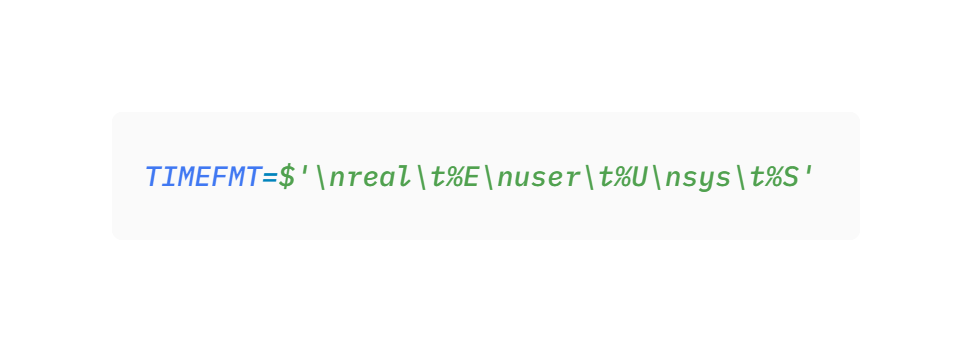
\includegraphics[width=0.8\textwidth]{time_command_format.png}
    \caption{Command to achieve desired output format}
\end{figure}

This command allows us to achieve the desired format. This is only necessary as we are using the Z-Shell, but the command itself 
still works the same as traditional Bash. Using the time command we can effectively measure the time that it takes from 
invocation to completion in a consistent format. This is a simple alternative to implementing a time measuring system into the 
SAT solver, which could potentially make it less performant. An example of the usage of the time command is shown below:

\begin{center}
    \texttt{\$ time make bin/dpll}
\end{center}

This command will invoke the 'make' binary to compile our program, called dpll. The output of this command will include both the 
output of the make command, as well as the time it took formatted to our previous rules:

% TODO: Improve the way this looks.
\begin{align*}
    \texttt{real: 4.70s} \\
    \texttt{user: 2.42s} \\
    \texttt{sys: 0.45s}
\end{align*}

% TODO: Make this picture look a bit better
%\begin{center}
%    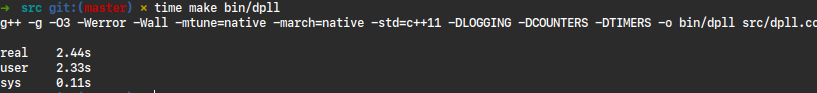
\includegraphics[scale=0.4]{time_command_example.png}
%\end{center}

\subsection{Final Program}
%\begin{itemize}
%    \item Investigate general pseudocode of generic DPLL algorithm (Wiki).
%    \item Create some pseudocode from algorithm.
%    \item Create some actual code to show?
%\end{itemize}
The final program works just as any other modern SAT solver would.
% TODO: Explain more about the final program.

\section{Testing}
%\begin{itemize}
%    \item Summarize what we want from the testing phase.
%    \item Discuss the problem sets that we are going to be throwing at this.
%    \item Discuss program testing first, even though this is not really what we mean by "testing".
%    \item Record some testing metrics, such as time to solve, memory, CPU cycles, etc.
%    \item Describe any regions that could potentially be improved.
%\end{itemize}
As with all software, one of the most important parts of the development lifecycle is testing. For
this project we must ensure that it not only works without fault, but also returns the correct
results that we are looking for. In order to test our software we shall generate a plethora of
testing criteria to test against. Each of these criteria will have an expected outcome. We will then
compare the expected outcome to the actual outcome and record whether they are identical. Although
this is a simple technique, it is hard to apply automated testing to our program as it is so niche.

As for ensuring the program returns correct results, the best way that we will be able to check is
to use well known and reputable solvers to generate results and compare the two. This can also be
added to the testing criteria and formatted in a table if preferred. The following will be the
details of the testing strategy alongside the results.

\subsection{Software Testing}
%\begin{itemize}
%    \item Discuss methods of software testing (Unit, manual, etc...)
%    \item Outline a testing table for manual testing.
%    \item Discuss testing against the functional requirements stated previously.
%\end{itemize}
There are a vast array of testing tools freely available to use for most software projects. These
have been created from the need for automated testing due to programs changing rapidly. In this
case, we do not need to deploy any advanced testing techniques or tools. As we have quite rigid
requirements and a small codebase, keeping track of changes is somewhat trivial. Much like discussed
in the initial sections of this paper, this is similar to the reasoning behind our choice of
methodology. Therefore, let us create a simple suite of manual testing criteria.

% TODO: Put a testing table here or something.

Now we can safely apply some of the traditional testing methodologies to our program.

\subsubsection{Unit Testing}
Unit testing is one of the most common types developers can use. This type of testing is where individual components or sections 
of the program are individually tested against a given criteria. Although there are multiple ways in which to achieve this, we do 
not need to overcomplicate this by writing hundreds of edge case tests. More importantly for this project, we only need to ensure 
that the program both compiles successfully, and produces the correct result.


\subsection{Checking For Correct Solutions}
%\begin{itemize}
%    \item Add results from test folder
%    \item Use two other solvers and give them the same problem
%    \item Check at least 10 times to ensure consistent results
%\end{itemize}
Progressing from the program testing, we must also ensure the solver is returning correct results.
This can also lead us to any bugs that may be present within the program. Using common SAT problems
presented in the DIMACS format we can compare the results from our program to results from another
solver. For statistical reasons we should ensure that each problem set is ran at least 10 times on
each solver. To further back up the testing results we could run the same problems against a third
solver. This would allow for comparison between each solver as a fall-back.

The first solver we will be using to ensure correctness is \textit{Minisat}. This solver is one of
the most tried and tested solvers freely available to use. And comes with plenty of features to
allow each test set to be completed quickly. \textit{Minisat} comes with a well documented interface
that we can use to easily build and run our test sets.

% TODO: Run our test set against Minisat. Record results here.

The fall-back solver we will be using is \textit{CryptoMiniSat}. This solver is still in active
development and encorporates some of the most advanced features for a FOSS solver. Compared to
\textit{Minisat}, this solver is significantly more complex. It should give us safe results that we
can use to ensure no descrepencies between our solver and \textit{Minisat}.

% TODO: Run our test set against CryptoMiniSat. Record results here.

Using the two mentioned solvers we can compare their results against our own. This is worth doing to make sure there are as 
little bugs as possible. The results for our testing are displayed below.

% TODO: Put the results from our solver here.

\subsection{Monitoring Initial Performance Metrics}
%\begin{itemize}
%    \item Measure the performance of this SAT solver (algorithm we picked?)
%    \item Measure the performance of other SAT solvers.
%    \item Compare the results and deduce why the performance differences exist.
%    \item Explain the use of the \texttt{'time'} command with special format.
%\end{itemize}

\subsubsection{UNIX Time Command}
There are multiple ways in which we could measure the performance of the solver. One easy way is
measuring the CPU time that the solver takes to give a solution to the problem it is given. This is
the reason we will be testing using the standard UNIX 'time' command. This command outputs three
metrics; real, user, and system. Real corresponds to the 'wall clock' time that the program took.
This refers to the actual time it took from invocation to completion whilst the CPU handles other
processes. The 'user' time corresponds to the time the CPU spent on the program in User mode. Calls
made in Kernel mode will not be reflected in this time. The 'sys' time corresponds to the time the
CPU spent in Kernel mode when executing the program. These three metrics give us a good idea as to
what the CPU spends the most time on when executing our program.

\subsubsection{Memory Usage}
Another method in which we can measure the performance of our solver is by keeping track of the
memory that is used. Although this may not seem like a performance related metric, it can tell us
about potential memory leaks which can in turn effect the general performance of the system. Aside
from this, it is important to keep track of the memory usage as a method of judging the solver
itself. Higher memory usage can indicate how many branches the solver is heading into before coming
to its solution. Typically more complex solvers that contain multiple algorithms, to solve
individual parts of the problem, can take up much less memory than a simpler one. The reason we add
more complexity is to ensure that the solver knows when it should stop trying to branch in a
particular direction. Less branching means we save a bit more memory and can sift through the
problem much quicker.

% TODO: Think about other ways of measuring performance.

\section{Results}
%\begin{itemize}
%    \item Discuss what we found from our testing
%\end{itemize}

\section{Evaluation}
%\begin{itemize}
%    \item Discuss our findings statistically.
%    \item Discuss how implemented code could be improved (summarise).
%    \item Talk about the methodology we used.
%    \item Talk about the risks encountered, and the time frame in which we carried this out.
%    \item Discuss the things that could potentially be improved if we did the project again.
%    \item Discuss the pandemic.
%\end{itemize}
\subsection{Accuracy}
One of the most important things to get right when creating this solver was to ensure the accuracy of the results. This is, after
all, the whole point of the solver in the first place. This can naturally be confirmed from our testing phase after the
implementation. By using alternative FOSS solvers we can clearly see that the implementation of Knuth's \textit{Algorithm L} works
just as intended. And as we will get into in the next section, performance is more than adequate. Of course, to ensure that this
implementation would be perfect across the whole range of potential problems it could face would take much longer. We would have
to collate a huge amount of problems and perhaps even test against the data sets that would be given at the SAT competition
itself. But for the intention of our project, and most importantly for the requirements we stated at the very beginning, this is
more than enough for our needs.

\subsection{Performance}
The second most important metric was the performance. Like stated above, we can draw from the requirements that we crafted at the
very start of the project. They proposed that the solver only has to be 'good enough', in the sense that it can solve most easy or
medium problems within a reasonable amount of time. 'Reasonable' is based off of the metrics of similar solvers in terms of
complexity. Of course, if we put this implementation against something like \textit{CryptoMiniSat} there is no chance that we
would be able to match its performance. What we could propose instead is taking the implementation of \textit{Algorithm L}, and
expanding on it by implementing experimental features, or taking inspiration from another solver such as \textit{CryptoMiniSat}
and implementing their ideas. This would of course take another project, and potentially much more time as the level of complexity
increases.

\subsection{Methodology}
The methodology used for this project turned out to be perfectly suitable, as intially thought. Like stated at the start, the
project goals and requirements were very rigid in theory, and in practice stayed consistent to that fact. We found no need to add
extra features, especially considering the task at hand was challenging enough. And if any features were deemed interesting to
add, that would be something for another project, as mentioned above. One thing to consider would be the possibility of starting
another project with another person, in which case the methodology we used may not be as suitable and would have to be discussed
in more detail.

\subsection{Implementation}
As for the implementation, we were fortunate to find that someone had already implemented all the algorithms from Knuth's booklet.
As these project files were hosted on GitHub\cite{aaw} and the license given was the \textit{Unlicense License}, we could freely
attain and modify this code for our own usage. This saved a huge amount of time, and after investigation, was found to have been
implemented in the exact way that Knuth had proposed. Potential improvements were made to this existing codebase by bringing
everything up to date with modern standards, and double checking that everything was working as intended. Of course, the resulting
program that we were interested in was only that of \textit{Algorithm L}. And as such, is the only included binary for this
project. The other binaries were used for testing purposes. As they are general implementations of each 'style' of common
algorithms, they proved to be a bonus when analysing the potential of each against \textit{Algorithm L}.

\section{Future Work}
%\begin{itemize}
%    \item Explore performance implications of algorithm.
%    \item Talk about DK's performance predictions from TAOCP.
%    \item Talk about how we could potentially improve the performance of our solver.
%    \item Maybe talk about things like parallelism?
%\end{itemize}

\subsection{Algorithm Performance}
There are multiple improvements that are suggested by Donald Knuth to speed up the initial DPLL algorithm based solver. The first 
of which is already listed as one of his alternative algorithms. Algorithm L uses the lookahead concept to substantially speed up 
the standard DPLL algorithm. This concept % TODO: Expand.

\subsection{Pre-processing}
One simple method that could greatly assist our solver is using a pre-processor. This will take the problem set and analyse it, 
and return a much simplified problem. This concept is applied accross modern solvers already, and is considered a vital part of 
the SAT solving system.

% TODO: Add some examples from existing solvers.

\subsection{Parallel Solving}
A more interesting concept is to capitalise on modern processor architectures, and the cheap availability of multi-core CPU's. It 
is commonplace to find consumer CPU's with at least 4 cores and hyper-threading. By taking advantage of this we can try to divide 
up the problem set and apply a solver to each smaller instance running on an individual thread. As usual with parallelism, this 
would not necessarily lead to a linear performance increase. It would require some research and engineering to determine the best 
way forward in order to achieve the desired results.

% TODO: Talk a bit more about this.

\subsection{SIMD}
Another interesting technique that could be applied to SAT solving is the use of SIMD instructions for data level parallelism. It 
has been shown in other applications that utilising SIMD instructions can quickly lead to almost linear performance improvements 
corresponding to each bit width of data processed. The most common SIMD instruction set is \textit{SSE} (Streaming SIMD 
Extensions). Introduced in 1999 by Intel, it is now commonplace is all modern consumer x86 processors. If there was a way to truly
implement SIMD into SAT solvers then there could be a massive potential for speedups in a range of applications. Even if the SIMD
instructions were implemented in auxilliary areas of the solver itself, it is worth the time to investigate the potential. 

% TODO: Maybe include some examples of SIMD in a solver?

\section{Challenges}
%\begin{itemize}
%    \item Discuss the challenges we faced.
%    \item Inlude the pandemic and associated issues.
%    \item Discuss how the nature of C++ can lead to confusion in development.
%    \item Discuss how a non-existent mathematical background made this \textit{very f*cking hard}.
%\end{itemize}
As with any project there will always be some challenges faced that skew the planned timeline. The following details the problems
that specifically effected this project and what could potentially be done to avoid facing these in the future.

\subsection{Software Based}
Implementing software will always come with its own set of challenges. Many projects have failed in the past for trivial reasons
associated with the software section not being fully understood. With this project, the main issue that we faced was with the
programming language itself, as detailed below.

\subsubsection{C++ Learning Curve}
The programming lanuage that was used for this project was deemed suitable based on the style of program to be created. SAT
solvers rely on heavy and intricate data structures to achieve what they need in the fastest time possible. Using C++ seemed like
a logical solution to this problem, as complex data structures can be created with ease. However, this does require some in-depth
knowledge of the language and its features first. C++ is notorious for being a language with a steep learning curve, and given the
time to learn it, ends up being one of the most powerful. The problem for this project was that prior in-depth knowledge of the
language was not known. This was thought of in the initial design of the project, but combined with the issues of a maths heavy
topic, proved to be more challenging that initially expected. 

\subsection{Project Based}
As stated above, most projects will face some form of setback or turmoil within their timescale. This project was no different,
and out of all the different forms of risks and setbacks that could have been encountered, one in particular stood out. However,
it would not be the only one that we could blame for this project not turning out as successful as intially hoped. There were a
few personal reasons which ended up causing much more damage to the time plan than intially thought. And on top of this,
over-ambition ended up playing a much bigger role than anticipated, as we will detail in the next few sections.

\subsubsection{Late Start}
One of the first challenges that had effected this project was the late start. This was in part due to both personal obligations 
that could not be avoided. As well as in part due to the Coronavirus pandemic. Although this did not effect the overall project 
progressing, it did push the establised timeframe beyond what had been originally planned. The domino effect of moving beyond the
allowed time buffer meant that each stage of the project had to be pushed back. Thus in turn creeping the expected deadline much
further back than anticipated.

\subsubsection{Coronavirus}
The second major issues encountered was something completely out of our control. The Coronavirus pandemic of 2020 provided a
massive slew of issues for all academia. Specifically for this project it meant the general plan for the project, as well as the
time plan, were both interrupted. The general lockdown for the United Kingdom resulted in confinement to the home. The
availability of face-to-face meetings proved to be unfavourable, and potential disruptions in the home delayed planned work.

\subsubsection{Maths Heavy Topic}
Another major issue encountered for this project was the lack of initial general mathematical background . This topic is a rather
maths heavy topic, with complex algorithms that can confuse most people who do not have strong mathematical skills. This lead to
this project being delayed in certain phases where more time had to be spent to understand the maths involved. Although in the end
this turned out to be good in the sense of challenging, the over-ambition to assume the ability to understand of all relevent
material turned against us. As such, in future projects there should be the advance knowledge of the required mathematical
background before starting. 

\section{Reflection}


\section{Conclusion}
\begin{itemize}
    \item Just make a short summary of every single thing that was typed out above!
    \item Don't forget to basically copy and paste this to the abstract.
\end{itemize}
% TODO: Conclude on our findings and all the preceding work we have done.
% === End Main Content ===

% === References ===
\newpage
\bibliographystyle{ieeetr}
\bibliography{references}
% === End References ===

\end{document}
